\chapter{Embedded System Architecture}
\label{chap:8}
In this chapter electronics architecture along with communication scheme is briefly explained. Complete close loop SGCMG unit is realised. Each individual SGCMG unit consist of a three phase close loop brushless motor driver to control reaction wheel at specified angular velocity with given angular acceleration signal. Gimbal motor is driven with Stepper Motor Driver and a dedicated micro-controller which provides appropriate signal to both motor drivers. Angular velocity of gimbal motor is measured using magnetic encoder. Communication protocol is implemented such that each SGCMG unit has dedicated address and returns angular velocity of reaction wheel, angle and angular velocity of gimbal motor when input desired states are provided. Body states of platform such as attitude quaternions, angular rates are computed from 3 axis IMU with dedicated on board master micro-controller for platform. Entire testbed architecture is divided in following major subsystems:
\begin{itemize}
    \item Platform Master State Feedback System
    \item Close Loop SGCMGs
    \item Electrical Power Systems
    \item Communication System
    \item Ground Control Station Server
\end{itemize}
\section{Platform Master State Feedback System}
Heart of testbench is master micro-controller has primary objective to evaluates platform orientation, body rates from an IMU and communicate in real time with Ground Control Station Server. It can also interact with other SGCMG units if VSCMG control is to be performed on board the platform.
\subsection{Microcontroller}
ESP32 an ultra low power MCU with integrated WiFi by Espressif Systems is used due to it's high performance dual core Tensilica Xtensa LX6 microprocessor running at 160 or 240 MHz, 39 GPIO and supports all standard embedded communication protocols such as 18 Analog-to-Digital Converter (ADC) channels, SPI, UART, I2C PWM output channels, Digital-to-Analog Converters (DAC) I2S interfaces etc, and requires very low power specifically 5V ~100mA(Max). \cite{web:ds_esp32}

\subsection{IMU}
Bosch Sensortech's BNO055 9 axis absolute orientation sensor is System in Package includes 3 axis 14-bit accelerometer, 3 axis magnetometer and 3 axis 16-bit gyroscope  and 32-bit microcontroller running on board sensor fusion algorithm.\cite{web:ds_BNO055}
\newacronym{mcu}{MCU}{Microcontroller Unit}
\newacronym{sda}{SDA}{Serial Data}
\newacronym{scl}{SCL}{Serial Clock}
\newacronym{pcb}{PCB}{Printed Circuit Board}
\noindent A custom  \acrshort{pcb} is designed in order to make sure proper and rigid placement of IMU and its interface with microcontroller. Schematic and PCB is shown in \autoref{fig:intefeceIMU} I2C protocol is used to communicate between \acrfull{mcu} and BNO055. \acrshort{sda} and \acrshort{scl} of BNO is connected to GPIO21 and GPIO22 of \acrshort{mcu}. Firmware inside \acrshort{mcu} is programmed in order to update and evaluate current angular velocity and orientation quaternions using Sebastian Madgwick's sensor fusion algorithm \cite{madgwick2010efficient} and send states to Ground station.

\begin{figure}[ht]
    \centering
    \begin{subfigure}[b]{0.4\textwidth}
         \centering
         \includegraphics[width=\textwidth]{figures/Electronics/intefeceSCH.pdf}
         \caption{Schematic diagram}
         \label{fig:intefeceSCH}
     \end{subfigure}
    \begin{subfigure}[b]{0.4\textwidth}
         \centering
         \includegraphics[width=\textwidth]{figures/Electronics/intefecePCB.pdf}
         \caption{Printed Circuit Board}
         \label{fig:intefecePCB}
     \end{subfigure}
    \caption{IMU interface board customized for BNO055 and ESP32. }
    \label{fig:intefeceIMU}
\end{figure}


\section{Close Loop SGCMG}
\begin{figure}[ht]
    \centering
    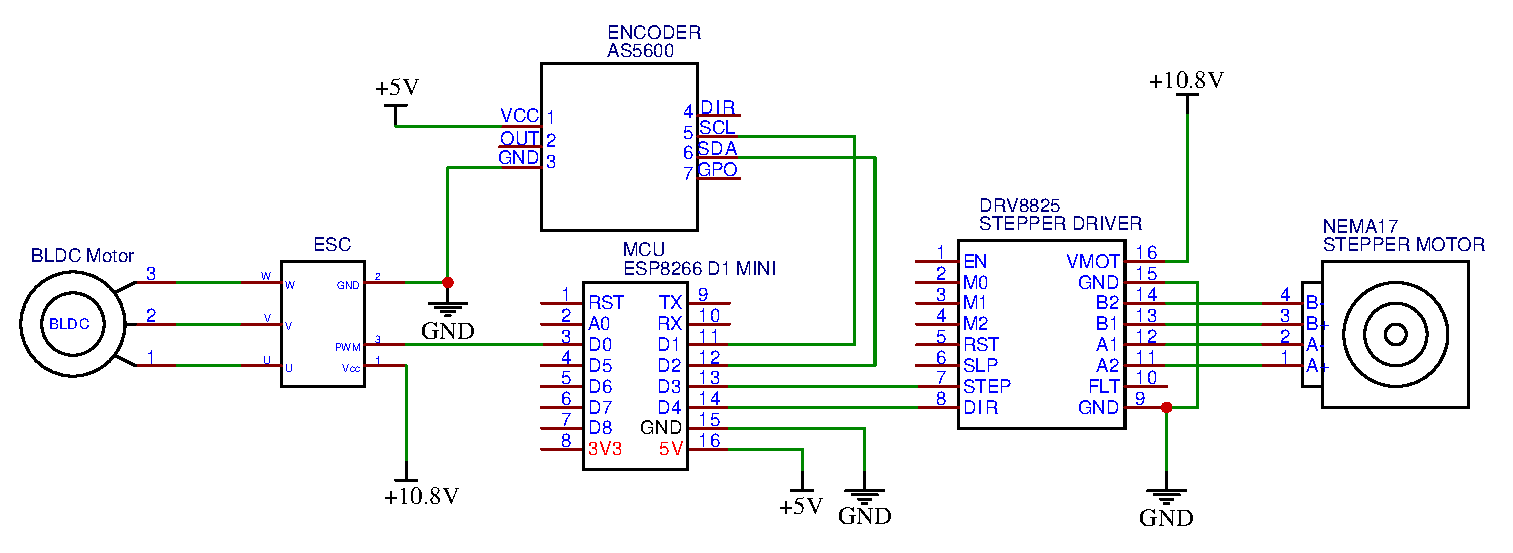
\includegraphics[width=\textwidth]{figures/Assembly/sgcmg_wiring.pdf}
    \caption{Schematic diagram of Close loop SGCMG electronics and wiring}
    \label{fig:sch_sgcmg_wiring}
\end{figure}
\section{Electrical Power System}
\section{Communication}

\begin{comment}


\section{Special commands provided by \textsf{sapthesis}}

\textsf{Sapthesis} provides some special commands, particularly useful for scientific works. You can use for example the roman shape, instead of the italic, for the imaginary unit (\texttt{\bs iu}) and Napier's number (\texttt{\bs eu}):
\begin{equation}
\eu^{\iu\pi}+1=0
\end{equation}

There are also two commands to speed up the writing of derivatives. In the following example we have used the commands \texttt{\bs der} and \texttt{\bs pder}):
\begin{equation}
\der{f}{x} \qquad \pder[2]{f}{y}
\end{equation}


\textsf{Sapthesis} provides also 4 commands to improve the writing of subscripts, \texttt{\bs rb} and \texttt{\bs tb}, and superscripts, \texttt{\bs rp} and \texttt{\bs tp}. Two of these commands, \texttt{\bs rb} and \texttt{\bs rp}, can be used both in text and in math mode and compose their argument in roman. The other two, \texttt{\bs tb} and \texttt{\bs tp}, can be used only in text mode and compose their argument as are. Here it is an usage example of \texttt{\bs rb} and \texttt{\bs rp}:
\[
a_b \neq a\rb{b}\qquad a^b \neq a\rp{b}
\]
And here it is an usage example of \texttt{\bs tb}: \emph{Cu\tb{It} indicates copper bought in Italy}. And a usage example of \texttt{\bs ts}: \emph{Cher G\tp{le} Napol\'eon}.


Then several commands for the correct typesetting of unit of measurements are provided. For example the command \texttt{\bs un} typesets its argument in roman and leaves a thin space between the number and the unit: $25\un{m}$, $3.5\un{m/s}$. Other commands are: (\texttt{\bs g}) 45\g, (\texttt{\bs C}) 30\,\C, (\texttt{\bs A}) 12\,\A, (\texttt{\bs micro}) 40\,\micro m, (\texttt{\bs ohm}) 27\,\ohm. 

We have also \texttt{\bs x} as abbreviation of \texttt{\bs times}: \$7 \bs x 10\^{}5\$ gives $7 \x 10^5$. Then \texttt{\bs di} is the differential symbol which automatically insert the correct spacing.
\[
\int x \di x
\]

Finally we have defined the color \textsf{sapred} which is the official color
of Sapienza -- University of Rome. It is defined as RGB(130,36,51). \textcolor{sapred}{This text is written with the color \textsf{sapred}.}
\marginpar{This is a fancy margin note!}
In the following dummy text you can observe the usage of \texttt{\bs mnote} command which typesets fancy margin notes.\cite{Baker2016}
\end{comment}
